\documentclass[12pt,english]{article}
\usepackage[a4paper,
            bindingoffset=0.2in,
            left=1in,
            right=1in,
            top=1in,
            bottom=1in,
            footskip=.25in]{geometry}
\usepackage{graphicx} % Required for inserting images
\usepackage[hidelinks]{hyperref}
\usepackage{array}
\usepackage{tabularx}
\usepackage{multirow}
\usepackage{xcolor}
\usepackage{tikz}
\usepackage{float}
\def\checkmark{\tikz\fill[scale=0.4](0,.35) -- (.25,0) -- (1,.7) -- (.25,.15) -- cycle;} 

\title{\textbf{SOEN 6431 \\ Software Comprehension and Maintenance}}
\author{Varun Pandey \\ Preet Angad Singh Nanda \\ Mir Pasad \\ Mahavir Patel }
\date{}

\begin{document}

\begin{figure}
    \centering
    
\includegraphics[width=10cm]{concordia.png}
\end{figure}
    
\maketitle
\vspace{3cm}
\begin{center}
    \huge{\textbf{Deliverable 2} \\ Re-engineering Operationalization}
\end{center}

\vspace{3cm}


\begin{center}
    \href{https://github.com/mahavir0/DEJA-VU---SOEN-6431-SCM}{\Large{https://github.com/DEJA-VU---SOEN-6431-SCM}}
\end{center}

\newpage

\tableofcontents

\newpage

\section{Abstract}
This document discusses the outcomes of a software re-engineering project aimed at improving a Java-based employee payroll system. The project sought to increase code maintainability and system future-proofing. This solution was chosen due to the team's comfort and the code's conformance to project criteria. To detect separate flaws in the code, two code analysis tools, Teamscale and SonarLint, were used. Teamscale was picked for its full analysis, which provided severity levels, precise locations, and potential solutions to the problems. Several undesired components, such as empty blocks, incorrect variable naming, and missing braces, were effectively rectified by the team. The efforts of re-engineering resulted in a well-structured codebase, ensuring the system's lifespan and improved functionality, allowing efficient tracking of remuneration and personnel information.

\section{Introduction}

Software Re-engineering is the process of making changes to a source code to make the code more maintainable and future proof. We have selected an employee payroll system for this project as mentioned in deliverable 1. 

\vspace{0.5cm}

The employee payroll system is programmed in Java and later the author has compiled an executable jar for this program. This is used to keep a track of the compensation and the employed department of each and every employee in the company. Once the project is executed we need to login using out admin credentials. For there we can view all the employees along with their relevant information. From there we can navigate to other windows where we can add new employees, edit existing employees, add and edit department information and add and edit admin credentials. 

\vspace{0.5cm}

The reason we chose this system is because this was the project all of us were most comfortable with amongst all the options. More detailed reasons can be found in deliverable 1. There were additional reason, such as the source code of R satisfied all the requirement as mentioned in the project description. The code was well written and structured, and therefore was it was easier for the team to read and understand the system. We chose 2 different software to audit our code, they are Teamscale and sonar-lint. The reason we chose 2 software is that we can later compare and contrast the results obtained from them and write our insights based on that. We then went through the code and each teammates was able to point out distinct issue with the code and later went on the fix those issues. 

\vspace{0.5cm}

The software re-engineering project focused on enhancing the Java-based employee payroll system has been successful. The system's selection was driven by the team's comfort and the code's adherence to project requirements. Through thorough code auditing using Teamscale and SonarLint, distinct issues were identified and effectively addressed. The re-engineering efforts have improved the system's maintainability and future-proofed its functionality. With a well-structured codebase, the payroll system now efficiently tracks compensation and employee department information, offering a user-friendly experience for administrators. Overall, the project's accomplishments have ensured the system's longevity and enhanced its performance.


\newpage
\section{Undesirable summary}

As mentioned in the introduction we used teamscale and sonar lint to audit the code, but after looking at the output we got from bother, we decided to go with teamscale's analysis because the teamscale was giving us more information about the errors, like severity level, location and possible fixes. Apart from that, teamscale also gave us better visuals for the issues. 


\begin{figure}[h!]
    \centering
    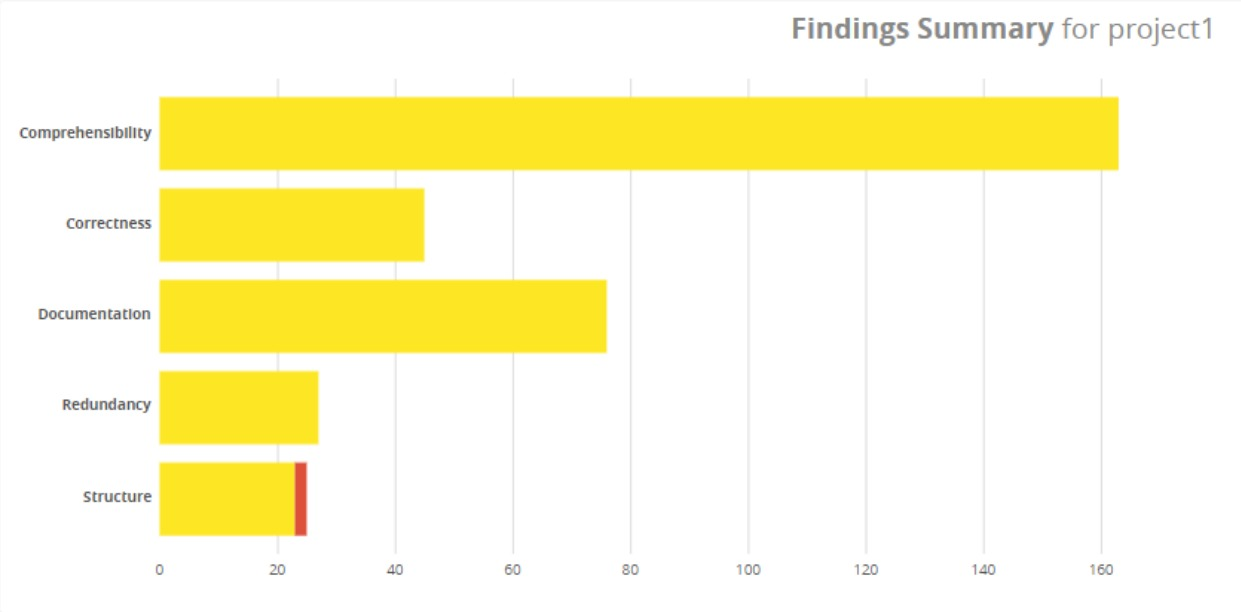
\includegraphics[width=15cm]{summary.jpeg}
\end{figure}


\begin{figure}[h!]
    % \centering
    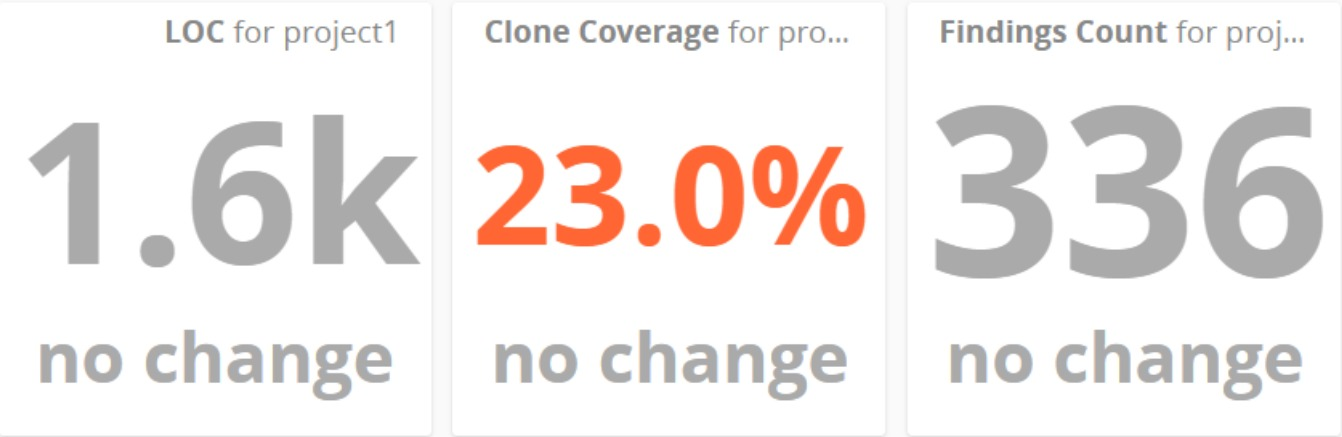
\includegraphics[width=15cm]{analytics.jpeg}
\end{figure}

\begin{figure}[h!]
    % \centering
    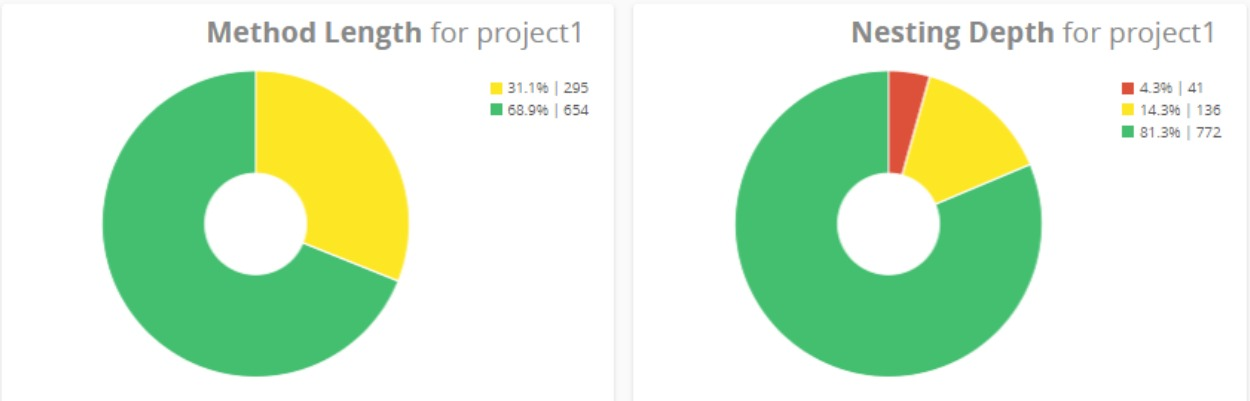
\includegraphics[width=15cm]{analytics2.jpeg}
\end{figure}

\begin{figure}[h!]
    % \centering
    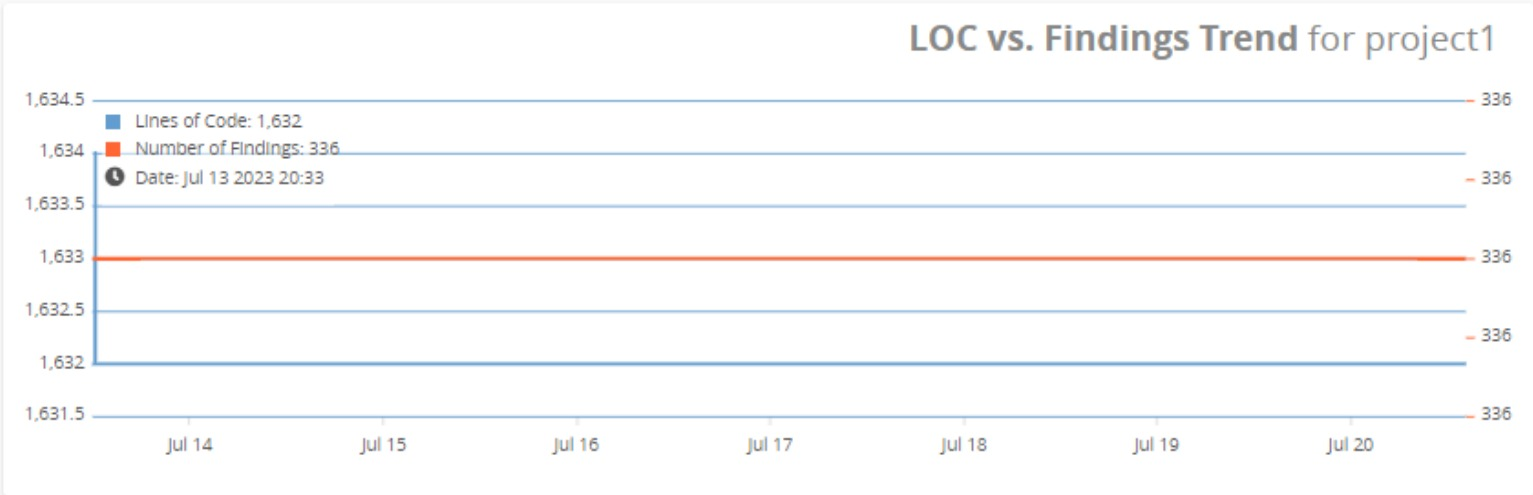
\includegraphics[width=15cm]{analytics3.jpeg}
    \caption{Lines of Code vs. Findings Trend of Candidate R - Employee Payroll System}
\end{figure}


\newpage

\begin{table}[!ht]
    \begin{tabularx}{\textwidth}{|c|l|X|}
    \hline
        \multirow{6}{*}{1} & Error Message & Empty block: method \\ \cline{2-3}
        & Occurrence & 3 \\ \cline{2-3}
        & Type & Bad Practice/case-empty-block \\ \cline{2-3}
        & Category & Comprehensibility \\ \cline{2-3}
        & Severity & Yellow \\ \cline{2-3}
        & Code Smell & Empty Catch Block \\ \hline
    \end{tabularx}
\end{table}

\begin{table}[!ht]
    \begin{tabularx}{\textwidth}{|c|l|X|}
    \hline
        \multirow{6}{*}{2} & Error Message & Static variable dbManager is not initialized \\ \cline{2-3}
        & Occurrence & 1 \\ \cline{2-3}
        & Type & Error-prone Practices \\ \cline{2-3}
        & Category & Correctness \\ \cline{2-3}
        & Severity & Yellow \\ \cline{2-3}
        & Code Smell & Code Quality \\ \hline
    \end{tabularx}
\end{table}

\begin{table}[!ht]
    \begin{tabularx}{\textwidth}{|c|l|X|}
    \hline
        \multirow{6}{*}{3} & Error Message & Attribute `btn\_delete` violates naming convention.*` \\ \cline{2-3}
        & Occurrence & 7 \\ \cline{2-3}
        & Type & Naming/JAVA \\ \cline{2-3}
        & Category & Comprehensibility \\ \cline{2-3}
        & Severity & Yellow \\ \cline{2-3}
        & Code Smell & Inconsistent Naming \\ \hline
    \end{tabularx}
\end{table}

\begin{table}[!ht]
    \begin{tabularx}{\textwidth}{|c|l|X|}
    \hline
        \multirow{6}{*}{4} & Error Message & Attribute `btn\_exit` violates naming convention.*` \\ \cline{2-3}
        & Occurrence & 1 \\ \cline{2-3}
        & Type & Naming/JAVA \\ \cline{2-3}
        & Category & Comprehensibility \\ \cline{2-3}
        & Severity & Yellow \\ \cline{2-3}
        & Code Smell & Inconsistent Naming \\ \hline
    \end{tabularx}
\end{table}

\begin{table}[!ht]
    \begin{tabularx}{\textwidth}{|c|l|X|}
    \hline
        \multirow{6}{*}{5} & Error Message & Non-constant public attribute dbManager \\ \cline{2-3}
        & Occurrence & 1 \\ \cline{2-3}
        & Type & Bad Practice \\ \cline{2-3}
        & Category & Comprehensibility \\ \cline{2-3}
        & Severity & Yellow \\ \cline{2-3}
        & Code Smell & Code quality  \\ \hline
    \end{tabularx}
\end{table}

\begin{table}[!ht]
    \begin{tabularx}{\textwidth}{|c|l|X|}
    \hline
        \multirow{6}{*}{6} & Error Message & Attribute `btn\_OK` violates naming convention.*` \\ \cline{2-3}
        & Occurrence & 1 \\ \cline{2-3}
        & Type & Naming/JAVA \\ \cline{2-3}
        & Category & Comprehensibility \\ \cline{2-3}
        & Severity & Yellow \\ \cline{2-3}
        & Code Smell & Inconsistent Naming \\ \hline
    \end{tabularx}
\end{table}

\begin{table}[!ht]
    \begin{tabularx}{\textwidth}{|c|l|X|}
    \hline
        \multirow{6}{*}{7} & Error Message & Attribute `btn\_update` violates naming convention.*` \\ \cline{2-3}
        & Occurrence & 1 \\ \cline{2-3}
        & Type & Naming/JAVA \\ \cline{2-3}
        & Category & Comprehensibility \\ \cline{2-3}
        & Severity & Yellow \\ \cline{2-3}
        & Code Smell & Inconsistent Naming \\ \hline
    \end{tabularx}
\end{table}

% \newpage

\begin{table}[!ht]
    \begin{tabularx}{\textwidth}{|c|l|X|}
    \hline
        \multirow{6}{*}{8} & Error Message & Method System.exit should not be called \\ \cline{2-3}
        & Occurrence & 2 \\ \cline{2-3}
        & Type & Discouraged APIs \\ \cline{2-3}
        & Category & Correctness \\ \cline{2-3}
        & Severity & Yellow \\ \cline{2-3}
        & Code Smell & Bug \\ \hline
    \end{tabularx}
\end{table}

\begin{table}[!ht]
    \begin{tabularx}{\textwidth}{|c|l|X|}
    \hline
        \multirow{6}{*}{9} & Error Message & Attribute `lbl\_basic\_salary` violates naming convention.*` \\ \cline{2-3}
        & Occurrence & 2 \\ \cline{2-3}
        & Type & Naming/JAVA \\ \cline{2-3}
        & Category & Comprehensibility \\ \cline{2-3}
        & Severity & Yellow \\ \cline{2-3}
        & Code Smell & Inconsistent Naming \\ \hline
    \end{tabularx}
\end{table}

\begin{table}[!ht]
    \begin{tabularx}{\textwidth}{|c|l|X|}
    \hline
        \multirow{6}{*}{10} & Error Message & Attribute `lbl\_da` violates naming convention.*` \\ \cline{2-3}
        & Occurrence & 2 \\ \cline{2-3}
        & Type & Naming/JAVA \\ \cline{2-3}
        & Category & Comprehensibility \\ \cline{2-3}
        & Severity & Yellow \\ \cline{2-3}
        & Code Smell & Inconsistent Naming \\ \hline
    \end{tabularx}
\end{table}

\begin{table}[!ht]
    \begin{tabularx}{\textwidth}{|c|l|X|}
    \hline
        \multirow{6}{*}{11} & Error Message & Attribute `lbl\_dep\_name` violates naming convention.*` \\ \cline{2-3}
        & Occurrence & 3 \\ \cline{2-3}
        & Type & Naming/JAVA \\ \cline{2-3}
        & Category & Comprehensibility \\ \cline{2-3}
        & Severity & Yellow \\ \cline{2-3}
        & Code Smell & Inconsistent Naming \\ \hline
    \end{tabularx}
\end{table}

\begin{table}[!ht]
    \begin{tabularx}{\textwidth}{|c|l|X|}
    \hline
        \multirow{6}{*}{12} & Error Message & Attribute `lbl\_department` violates naming convention.*` \\ \cline{2-3}
        & Occurrence & 2 \\ \cline{2-3}
        & Type & Naming/JAVA \\ \cline{2-3}
        & Category & Comprehensibility \\ \cline{2-3}
        & Severity & Yellow \\ \cline{2-3}
        & Code Smell & Inconsistent Naming \\ \hline
    \end{tabularx}
\end{table}

\begin{table}[!ht]
    \begin{tabularx}{\textwidth}{|c|l|X|}
    \hline
        \multirow{6}{*}{13} & Error Message & Attribute `lbl\_em` violates naming convention.*` \\ \cline{2-3}
        & Occurrence & 2 \\ \cline{2-3}
        & Type & Naming/JAVA \\ \cline{2-3}
        & Category & Comprehensibility \\ \cline{2-3}
        & Severity & Yellow \\ \cline{2-3}
        & Code Smell & Inconsistent Naming \\ \hline
    \end{tabularx}
\end{table}

\begin{table}[!ht]
    \begin{tabularx}{\textwidth}{|c|l|X|}
    \hline
        \multirow{6}{*}{14} & Error Message & Clone with 2 instances of length x \\ \cline{2-3}
        & Occurrence & 27 \\ \cline{2-3}
        & Type & Redundancy/Clones \\ \cline{2-3}
        & Category & Redundancy \\ \cline{2-3}
        & Severity & Yellow \\ \cline{2-3}
        & Code Smell & Insufficient Abstraction \\ \hline
    \end{tabularx}
\end{table}

\begin{table}[!ht]
    \begin{tabularx}{\textwidth}{|c|l|X|}
    \hline
        \multirow{6}{*}{15} & Error Message & else statement without braces \\ \cline{2-3}
        & Occurrence & 8 \\ \cline{2-3}
        & Type & Error-prone Practices \\ \cline{2-3}
        & Category & Correctness \\ \cline{2-3}
        & Severity & Yellow \\ \cline{2-3}
        & Code Smell & Missing Braces \\ \hline
    \end{tabularx}
\end{table}

% \newpage

\begin{table}[!ht]
    \begin{tabularx}{\textwidth}{|c|l|X|}
    \hline
        \multirow{6}{*}{16} & Error Message & if statement without braces \\ \cline{2-3}
        & Occurrence & 13 \\ \cline{2-3}
        & Type & Error-prone Practices \\ \cline{2-3}
        & Category & Correctness \\ \cline{2-3}
        & Severity & Yellow \\ \cline{2-3}
        & Code Smell & Missing Braces \\ \hline
    \end{tabularx}
\end{table}

\begin{table}[!ht]
    \begin{tabularx}{\textwidth}{|c|l|X|}
    \hline
        \multirow{6}{*}{17} & Error Message & Interface comment missing \\ \cline{2-3}
        & Occurrence & 75 \\ \cline{2-3}
        & Type & Comments/Missing Interface Comment \\ \cline{2-3}
        & Category & Documentation \\ \cline{2-3}
        & Severity & Yellow \\ \cline{2-3}
        & Code Smell & Missing Documentation \\ \hline
    \end{tabularx}
\end{table}

\begin{table}[!ht]
    \begin{tabularx}{\textwidth}{|c|l|X|}
    \hline
        \multirow{6}{*}{18} & Error Message & Method `System.err.println` should not be called \\ \cline{2-3}
        & Occurrence & 20 \\ \cline{2-3}
        & Type & Discouraged APIs \\ \cline{2-3}
        & Category & Correctness \\ \cline{2-3}
        & Severity & Yellow \\ \cline{2-3}
        & Code Smell & Standard Output/Error Usage \\ \hline
    \end{tabularx}
\end{table}

\begin{table}[!ht]
    \begin{tabularx}{\textwidth}{|c|l|X|}
    \hline
        \multirow{6}{*}{19} & Error Message & Violation of nesting depth threshold of 3: 4 \\ \cline{2-3}
        & Occurrence & 15 \\ \cline{2-3}
        & Type & Metric Violations/Nesting Depth \\ \cline{2-3}
        & Category & Structure \\ \cline{2-3}
        & Severity & Yellow \\ \cline{2-3}
        & Code Smell & Excessive Nesting \\ \hline
    \end{tabularx}
\end{table}

\begin{table}[!ht]
    \begin{tabularx}{\textwidth}{|c|l|X|}
    \hline
        \multirow{6}{*}{20} & Error Message & Violation of method length threshold (source lines of code) of x:y \\ \cline{2-3}
        & Occurrence & 10 \\ \cline{2-3}
        & Type & Metric Violations/LSL \\ \cline{2-3}
        & Category & Structure \\ \cline{2-3}
        & Severity & Yellow \\ \cline{2-3}
        & Code Smell & Long Method \\ \hline
    \end{tabularx}
\end{table}

\begin{table}[!ht]
    \begin{tabularx}{\textwidth}{|c|l|X|}
    \hline
        \multirow{6}{*}{21} & Error Message & Star import of `java.awt.*` should not be used \\ \cline{2-3}
        & Occurrence & 11 \\ \cline{2-3}
        & Type & Bad Practice \\ \cline{2-3}
        & Category & Comprehensibility \\ \cline{2-3}
        & Severity & Yellow \\ \cline{2-3}
        & Code Smell & Wildcard Import \\ \hline
    \end{tabularx}
\end{table}

\begin{table}[!ht]
    \begin{tabularx}{\textwidth}{|c|l|X|}
    \hline
        \multirow{6}{*}{22} & Error Message & Star import of `java.awt.event.*` should not be used \\ \cline{2-3}
        & Occurrence & 11 \\ \cline{2-3}
        & Type & Bad Practice \\ \cline{2-3}
        & Category & Comprehensibility \\ \cline{2-3}
        & Severity & Yellow \\ \cline{2-3}
        & Code Smell & Wildcard Import \\ \hline
    \end{tabularx}
\end{table}


\begin{table}[!ht]
    \begin{tabularx}{\textwidth}{|c|l|X|}
    \hline
        \multirow{6}{*}{23} & Error Message & Star import of `javax.swing.*` should not be used \\ \cline{2-3}
        & Occurrence & 11 \\ \cline{2-3}
        & Type & Bad Practice \\ \cline{2-3}
        & Category & Comprehensibility \\ \cline{2-3}
        & Severity & Yellow \\ \cline{2-3}
        & Code Smell & Wildcard Import \\ \hline
    \end{tabularx}
\end{table}

\begin{table}[!ht]
    \begin{tabularx}{\textwidth}{|c|l|X|}
    \hline
        \multirow{6}{*}{24} & Error Message & Star import of `org.payroll.*` should not be used \\ \cline{2-3}
        & Occurrence & 9 \\ \cline{2-3}
        & Type & Bad Practice \\ \cline{2-3}
        & Category & Comprehensibility \\ \cline{2-3}
        & Severity & Yellow \\ \cline{2-3}
        & Code Smell & Wildcard Import \\ \hline
    \end{tabularx}
\end{table}

% \newpage

\begin{table}[!ht]
    \begin{tabularx}{\textwidth}{|c|l|X|}
    \hline
        \multirow{6}{*}{25} & Error Message & Star import of `java.util.*` should not be used \\ \cline{2-3}
        & Occurrence & 6 \\ \cline{2-3}
        & Type & Bad Practice \\ \cline{2-3}
        & Category & Comprehensibility \\ \cline{2-3}
        & Severity & Yellow \\ \cline{2-3}
        & Code Smell & Wildcard Import \\ \hline
    \end{tabularx}
\end{table}
\clearpage

\newpage

\section{ Re-engineering Methods for Undesirables}
We demonstrated our findings in this area and related them to their reengineering rule, reengineering rule type, rule tag, undesirable severity, unfavourable likelihood, and the name of the team member who refactored it. For the most part, this information was obtained via evaluating the following forum https://rules.sonarsource.com/java and mapping the discovery to the best-fitting reengineering rule.

\begin{table}[!ht]
    \begin{tabularx}{\textwidth}{|c|c|X|}
    \hline
        \multirow{7}{*}{1} & Findings & Empty block: method \\ \cline{2-3}
        & Re-engineering Rule Description & For a number of reasons, a method may not have a method body.
        Unintentional mistakes ought to be fixed, as this one is.
        It is not now and never will be supported. 
        The override method is intentionally empty. In this situation, a nested comment must give a justification for the blank.
 \\ \cline{2-3}
        & Re-engineering Rule Type & Code Smell \\ \cline{2-3}
        & Rule Tag & Suspicious \\ \cline{2-3}
        & Undesirable Severity & Yellow \\ \cline{2-3}
        & Undesirable Likelihood & Low \\ \cline{2-3}
        & Refactored By & Mahavir Patel \\ \hline
    \end{tabularx}
\end{table}

\begin{table}[!ht]
    \begin{tabularx}{\textwidth}{|c|l|X|}
    \hline
        \multirow{7}{*}{2} & Findings & Static variable dbManager is not initialized \\ \cline{2-3}
        & Re-engineering Rule Description & Ensure that all static variables, including dbManager, are initialized before they are accessed or used. Proper initialization prevents potential runtime errors and guarantees that static variables have valid values at all times. \\ \cline{2-3}
        & Re-engineering Rule Type & Vulnerability \\ \cline{2-3}
        & Rule Tag & Major \\ \cline{2-3}
        & Undesirable Severity & Yellow \\ \cline{2-3}
        & Undesirable Likelihood & Low \\ \cline{2-3}
        & Refactored By & Mahavir Patel \\ \hline
    \end{tabularx}
\end{table}

\begin{table}[!ht]
    \begin{tabularx}{\textwidth}{|c|l|X|}
    \hline
        \multirow{7}{*}{3} & Findings & Attribute ‘btn delete‘ violates naming convention.*‘ \\ \cline{2-3}
        & Re-engineering Rule Description & Teams may work together effectively using shared coding norms. This rule determines if every constant name satisfies the given regular expression.
 \\ \cline{2-3}
        & Re-engineering Rule Type & Code Smell \\ \cline{2-3}
        & Rule Tag & Convention \\ \cline{2-3}
        & Undesirable Severity & Yellow \\ \cline{2-3}
        & Undesirable Likelihood & Medium \\ \cline{2-3}
        & Refactored By & Mahavir Patel \\ \hline
    \end{tabularx}
\end{table}

\begin{table}[!ht]
    \begin{tabularx}{\textwidth}{|c|l|X|}
    \hline
        \multirow{7}{*}{4} & Findings & Attribute ‘btn exit‘ violates naming convention.*‘ \\ \cline{2-3}
        & Re-engineering Rule Description & Teams may work together effectively using shared coding norms. This rule determines if every constant name satisfies the given regular expression.
        \\ \cline{2-3}
        & Re-engineering Rule Type & Code Smell  \\ \cline{2-3}
        & Rule Tag & Convention \\ \cline{2-3}
        & Undesirable Severity & Yellow \\ \cline{2-3}
        & Undesirable Likelihood & Low \\ \cline{2-3}
        & Refactored By & Mahavir Patel \\ \hline
    \end{tabularx}
\end{table}

\begin{table}[!ht]
    \begin{tabularx}{\textwidth}{|c|l|X|}
    \hline
        \multirow{7}{*}{5} & Findings & Non-constant public attribute dbManager \\ \cline{2-3}
        & Re-engineering Rule Description & Class attributes, such as dbManager, should be declared as private or protected, and access to them should be provided through getter and setter methods. Avoid exposing class attributes directly as public to ensure proper encapsulation and maintain data integrity. \\ \cline{2-3}
        & Re-engineering Rule Type & Vulnerability \\ \cline{2-3}
        & Rule Tag & Major \\ \cline{2-3}
        & Undesirable Severity & Yellow \\ \cline{2-3}
        & Undesirable Likelihood & Low \\ \cline{2-3}
        & Refactored By & Mahavir Patel \\ \hline
    \end{tabularx}
\end{table}

\begin{table}[!ht]
    \begin{tabularx}{\textwidth}{|c|l|X|}
    \hline
        \multirow{7}{*}{6} & Findings & Attribute ‘btn OK‘ violates naming convention.*‘ \\ \cline{2-3}
        & Re-engineering Rule Description & Teams may work together effectively using shared coding norms. This rule determines if every constant name satisfies the given regular expression.
        \\ \cline{2-3}
        & Re-engineering Rule Type & Code Smell \\ \cline{2-3}
        & Rule Tag & Convention \\ \cline{2-3}
        & Undesirable Severity & Yellow \\ \cline{2-3}
        & Undesirable Likelihood & Low \\ \cline{2-3}
        & Refactored By  & Mahavir Patel \\ \hline
    \end{tabularx}
\end{table}

\begin{table}[!ht]
    \begin{tabularx}{\textwidth}{|c|l|X|}
    \hline
        \multirow{7}{*}{7} & Findings & Attribute ‘btn update‘ violates naming convention.*‘ \\ \cline{2-3}
        & Re-engineering Rule Description & Teams may work together effectively using shared coding norms. This rule determines if every constant name satisfies the given regular expression.\\ \cline{2-3}
        & Re-engineering Rule Type & Code Smell  \\ \cline{2-3}
        & Rule Tag & Convention \\ \cline{2-3}
        & Undesirable Severity & Yellow \\ \cline{2-3}
        & Undesirable Likelihood & Low \\ \cline{2-3}
        & Refactored By & Preet Angad Singh Nanda \\ \hline
    \end{tabularx}
\end{table}

\begin{table}[!ht]
    \begin{tabularx}{\textwidth}{|c|l|X|}
    \hline
        \multirow{7}{*}{8} & Findings & Method System.exit should not be called \\ \cline{2-3}
        & Re-engineering Rule Description & There are several implementation classes available for interfaces to meet different needs. Specified performance aspects are guaranteed by some implementations, whereas specified behaviours, such immutability, are guaranteed by others.
        Therefore, before invoking a "optional" method, a developer should make sure that the implementation class on which the call is made implements it.

\\ \cline{2-3}
        & Re-engineering Rule Type & Bug \\ \cline{2-3}
        & Rule Tag & N/A \\ \cline{2-3}
        & Undesirable Severity & Yellow \\ \cline{2-3}
        & Undesirable Likelihood & Low \\ \cline{2-3}
        & Refactored By & Preet Angad Singh Nanda \\ \hline
    \end{tabularx}
\end{table}

\begin{table}[!ht]
    \begin{tabularx}{\textwidth}{|c|l|X|}
    \hline
        \multirow{7}{*}{9} & Findings & Attribute ‘lbl basic salary‘ violates naming convention.*‘ \\ \cline{2-3}
        & Re-engineering Rule Description & Teams may work together effectively using shared coding norms. This rule determines if every constant name satisfies the given regular expression.\\ \cline{2-3}
        & Re-engineering Rule Type & Code Smell \\ \cline{2-3}
        & Rule Tag & Convention \\ \cline{2-3}
        & Undesirable Severity & Yellow \\ \cline{2-3}
        & Undesirable Likelihood & Low \\ \cline{2-3}
        & Refactored By & Preet Angad Singh Nanda \\ \hline
    \end{tabularx}
\end{table}

\begin{table}[!ht]
    \begin{tabularx}{\textwidth}{|c|l|X|}
    \hline
        \multirow{7}{*}{10} & Findings & Attribute ‘lbl da‘ violates naming convention.* \\ \cline{2-3}
        & Re-engineering Rule Description & Teams may work together effectively using shared coding norms. This rule determines if every constant name satisfies the given regular expression. \\ \cline{2-3}
        & Re-engineering Rule Type & Code Smell \\ \cline{2-3}
        & Rule Tag & Convention \\ \cline{2-3}
        & Undesirable Severity & Yellow \\ \cline{2-3}
        & Undesirable Likelihood & Low \\ \cline{2-3}
        & Refactored By & Preet Angad Singh Nanda \\ \hline
    \end{tabularx}
\end{table}

\begin{table}[!ht]
    \begin{tabularx}{\textwidth}{|c|l|X|}
    \hline
        \multirow{7}{*}{11} & Findings & Attribute ‘lbl dep name‘ violates naming convention.*‘ \\ \cline{2-3}
        & Re-engineering Rule Description & Teams may work together effectively using shared coding norms. This rule determines if every constant name satisfies the given regular expression.
 \\ \cline{2-3}
        & Re-engineering Rule Type & Code Smell \\ \cline{2-3}
        & Rule Tag & Convention \\ \cline{2-3}
        & Undesirable Severity & Yellow \\ \cline{2-3}
        & Undesirable Likelihood & Low \\ \cline{2-3}
        & Refactored By & Preet Angad Singh Nanda \\ \hline
    \end{tabularx}
\end{table}

\begin{table}[!ht]
    \begin{tabularx}{\textwidth}{|c|l|X|}
    \hline
        \multirow{7}{*}{12} & Findings & Attribute ‘lbl department‘ violates naming convention.*‘ \\ \cline{2-3}
        & Re-engineering Rule Description & Teams may work together effectively using shared coding norms. This rule determines if every constant name satisfies the given regular expression.
 \\ \cline{2-3}
        & Re-engineering Rule Type & Code Smell \\ \cline{2-3}
        & Rule Tag & Convention \\ \cline{2-3}
        & Undesirable Severity & Yellow \\ \cline{2-3}
        & Undesirable Likelihood & Low \\ \cline{2-3}
        & Refactored By & Preet Angad Singh Nanda \\ \hline
    \end{tabularx}
\end{table}

\begin{table}[!ht]
    \begin{tabularx}{\textwidth}{|c|l|X|}
    \hline
        \multirow{7}{*}{13} & Findings & Attribute ‘lbl em‘ violates naming convention.*‘ \\ \cline{2-3}
        & Re-engineering Rule Description & Teams may work together effectively using shared coding norms. This rule determines if every constant name satisfies the given regular expression.
 \\ \cline{2-3}
        & Re-engineering Rule Type & Code Smell \\ \cline{2-3}
        & Rule Tag & Convention \\ \cline{2-3}
        & Undesirable Severity & Yellow \\ \cline{2-3}
        & Undesirable Likelihood & Low \\ \cline{2-3}
        & Refactored By & Varun Pandey \\ \hline
    \end{tabularx}
\end{table}

\begin{table}[!ht]
    \begin{tabularx}{\textwidth}{|c|l|X|}
    \hline
        \multirow{7}{*}{14} & Findings & Clone with 2 instances of length x \\ \cline{2-3}
        & Re-engineering Rule Description & It should not be changed to "clone"
 \\ \cline{2-3}
        & Re-engineering Rule Type & Code Smell \\ \cline{2-3}
        & Rule Tag & Suspicious
 \\ \cline{2-3}
        & Undesirable Severity & Yellow \\ \cline{2-3}
        & Undesirable Likelihood & High \\ \cline{2-3}
        & Refactored By & Varun Pandey \\ \hline
    \end{tabularx}
\end{table}

\begin{table}[!ht]
    \begin{tabularx}{\textwidth}{|c|l|X|}
    \hline
        \multirow{7}{*}{15} & Findings & else statement without braces \\ \cline{2-3}
        & Re-engineering Rule Description &  It can lead to confusion and unintended consequences, especially when developers later modify the code by adding more statements to the conditional branch. Code must consistently enclose the body of an else statement with braces, even if it contains only a single statement. This ensures code readability, avoids potential bugs due to indentation issues, and future-proofs the code against unintended side effects when modifying the conditional branch.  \\ \cline{2-3}
        & Re-engineering Rule Type & Code Quality \\ \cline{2-3}
        & Rule Tag & Minor \\ \cline{2-3}
        & Undesirable Severity & Yellow \\ \cline{2-3}
        & Undesirable Likelihood & Low \\ \cline{2-3}
        & Refactored By & Varun Pandey \\ \hline
    \end{tabularx}
\end{table}

\begin{table}[!ht]
    \begin{tabularx}{\textwidth}{|c|l|X|}
    \hline
        \multirow{7}{*}{16} & Findings & if statement without braces \\ \cline{2-3}
        & Re-engineering Rule Description & It can lead to confusion and unintended consequences, especially when developers later modify the code by adding more statements to the conditional branch. Code must consistently enclose the body of an if statement with braces, even if it contains only a single statement. This ensures code readability, avoids potential bugs due to indentation issues, and future-proofs the code against unintended side effects when modifying the conditional branch.  \\ \cline{2-3}
        & Re-engineering Rule Type & Code Quality \\ \cline{2-3}
        & Rule Tag & Minor \\ \cline{2-3}
        & Undesirable Severity & Yellow \\ \cline{2-3}
        & Undesirable Likelihood & Medium \\ \cline{2-3}
        & Refactored By & Varun Pandey \\ \hline
    \end{tabularx}
\end{table}

\begin{table}[!ht]
    \begin{tabularx}{\textwidth}{|c|l|X|}
    \hline
        \multirow{7}{*}{17} & Findings & Interface comment missing \\ \cline{2-3}
        & Re-engineering Rule Description & There is no JavaDoc accessible for the models, interfaces, or classes.
  \\ \cline{2-3}
        & Re-engineering Rule Type & Code Smell \\ \cline{2-3}
        & Rule Tag & Unused \\ \cline{2-3}
        & Undesirable Severity & Yellow \\ \cline{2-3}
        & Undesirable Likelihood & High \\ \cline{2-3}
        & Refactored By & Varun Pandey \\ \hline
    \end{tabularx}
\end{table}

\begin{table}[!ht]
    \begin{tabularx}{\textwidth}{|c|l|X|}
    \hline
        \multirow{7}{*}{18} & Findings & Method ‘System.err.println‘ should not be called \\ \cline{2-3}
        & Re-engineering Rule Description & There are several implementation classes available for interfaces to meet different needs. Specified performance aspects are guaranteed by some implementations, whereas specified behaviours, such immutability, are guaranteed by others.
        Therefore, before invoking a "optional" method, a developer should make sure that the implementation class on which the call is made implements it.
 \\ \cline{2-3}
        & Re-engineering Rule Type & Bug \\ \cline{2-3}
        & Rule Tag & N/A \\ \cline{2-3}
        & Undesirable Severity & Yellow \\ \cline{2-3}
        & Undesirable Likelihood & Medium \\ \cline{2-3}
        & Refactored By & Varun Pandey \\ \hline
    \end{tabularx}
\end{table}

\begin{table}[!ht]
    \begin{tabularx}{\textwidth}{|c|l|X|}
    \hline
        \multirow{7}{*}{19} & Findings & Violation of nesting depth threshold of 3: 4 \\ \cline{2-3}
        & Re-engineering Rule Description & Excessive nesting can lead to code that is harder to read, understand, and maintain. It can also increase the chances of introducing bugs and make the code more challenging to modify or refactor in the future. \\ \cline{2-3}
        & Re-engineering Rule Type & Bugs \\ \cline{2-3}
        & Rule Tag & Checkstyle \\ \cline{2-3}
        & Undesirable Severity & Yellow \\ \cline{2-3}
        & Undesirable Likelihood & Medium \\ \cline{2-3}
        & Refactored By & Mir Pasad \\ \hline
    \end{tabularx}
\end{table}

\begin{table}[!ht]
    \begin{tabularx}{\textwidth}{|c|l|X|}
    \hline
        \multirow{7}{*}{20} & Findings & Violation of method length threshold (source lines of code) of
x:y \\ \cline{2-3}
        & Re-engineering Rule Description & a particular method in the codebase has exceeded the allowed or recommended length limit set by the coding standards or guidelines of the project. It may also be an indicator that the method is doing too much and should be refactored into smaller, more focused methods with clear responsibilities.  \\ \cline{2-3}
        & Re-engineering Rule Type & Code Smell \\ \cline{2-3}
        & Rule Tag & Checkstyle \\ \cline{2-3}
        & Undesirable Severity & Yellow \\ \cline{2-3}
        & Undesirable Likelihood & Medium \\ \cline{2-3}
        & Refactored By & Mir Pasad \\ \hline
    \end{tabularx}
\end{table}

\begin{table}[!ht]
    \begin{tabularx}{\textwidth}{|c|l|X|}
    \hline
        \multirow{7}{*}{21} & Findings & Star import of ‘java.awt.*‘ should not be used \\ \cline{2-3}
        & Re-engineering Rule Description & Similar to database queries, using wildcards to import software libraries or packages may be a sign of laziness on the part of individuals who don't want to take the effort to import a specific component (such as import java.awt.*) to be utilised in their program.  Too many wildcard imports might result in problems when your programs are being compiled.
 \\ \cline{2-3}
        & Re-engineering Rule Type & Vulnerability \\ \cline{2-3}
        & Rule Tag & Slow Compilation \\ \cline{2-3}
        & Undesirable Severity & Yellow \\ \cline{2-3}
        & Undesirable Likelihood & Medium \\ \cline{2-3}
        & Refactored By & Mir Pasad \\ \hline
    \end{tabularx}
\end{table}

\begin{table}[!ht]
    \begin{tabularx}{\textwidth}{|c|l|X|}
    \hline
        \multirow{7}{*}{22} & Findings & Star import of ‘java.awt.event.*‘ should not be used \\ \cline{2-3}
        & Re-engineering Rule Description & Similar to database queries, using wildcards to import software libraries or packages may be a sign of laziness on the part of individuals who don't want to take the effort to import a specific component (such as import java.awt.Event.*) to be utilised in their program.  Too many wildcard imports might result in problems when your programs are being compiled.
 \\ \cline{2-3}
        & Re-engineering Rule Type & Vulnerability \\ \cline{2-3}
        & Rule Tag & Slow Compilation \\ \cline{2-3}
        & Undesirable Severity & Yellow \\ \cline{2-3}
        & Undesirable Likelihood & Medium \\ \cline{2-3}
        & Refactored By & Mir Pasad \\ \hline
    \end{tabularx}
\end{table}

\begin{table}[!ht]
    \begin{tabularx}{\textwidth}{|c|l|X|}
    \hline
        \multirow{7}{*}{23} & Findings & Star import of ‘javax.swing.*‘ should not be used \\ \cline{2-3}
        & Re-engineering Rule Description & Similar to database queries, using wildcards to import software libraries or packages may be a sign of laziness on the part of individuals who don't want to take the effort to import a specific component (such as import java.swing.*) to be utilised in their program.  Too many wildcard imports might result in problems when your programs are being compiled.
 \\ \cline{2-3}
        & Re-engineering Rule Type & Vulnerability \\ \cline{2-3}
        & Rule Tag & Slow Compilation \\ \cline{2-3}
        & Undesirable Severity & Yellow \\ \cline{2-3}
        & Undesirable Likelihood & Medium \\ \cline{2-3}
        & Refactored By & Mir Pasad \\ \hline
    \end{tabularx}
\end{table}

\begin{table}[!ht]
    \begin{tabularx}{\textwidth}{|c|l|X|}
    \hline
        \multirow{7}{*}{24} & Findings & Star import of ‘org.payroll.*‘ should not be used \\ \cline{2-3}
        & Re-engineering Rule Description & Java programs compile-time speed could be somewhat impacted by the use of wildcard imports, but runtime performance won't be impacted at all. When it comes to clean coding, you have to be careful how you employ it.
. \\ \cline{2-3}
        & Re-engineering Rule Type & Vulnerability \\ \cline{2-3}
        & Rule Tag & Slow Compilation  \\ \cline{2-3}
        & Undesirable Severity & Yellow \\ \cline{2-3}
        & Undesirable Likelihood & Low \\ \cline{2-3}
        & Refactored By & Mir Pasad \\ \hline
    \end{tabularx}
\end{table}

\begin{table}[!ht]
    \begin{tabularx}{\textwidth}{|c|l|X|}
    \hline
        \multirow{7}{*}{25} & Findings & Star import of ‘java.util.*‘ should not be used \\ \cline{2-3}
        & Re-engineering Rule Description & Java programs compile-time speed could be somewhat impacted by the use of wildcard imports, but runtime performance won't be impacted at all. When it comes to clean coding, you have to be careful how you employ it.
 \\ \cline{2-3}
        & Re-engineering Rule Type & Vulnerability \\ \cline{2-3}
        & Rule Tag & Slow Compilation \\ \cline{2-3}
        & Undesirable Severity & Yellow \\ \cline{2-3}
        & Undesirable Likelihood & Low \\ \cline{2-3}
        & Refactored By & Mir Pasad \\ \hline
    \end{tabularx}
\end{table}

\clearpage
\newpage

\section{ Location of Source code Undesirables}
The table below summarises all of the undesirable sites. The location of the undesirable is indicated by saying the folder name, then the file where it is found within this folder, and where this undesirable is found, as well as how many lines of source code it contains.

\begin{table}[!ht]
    \begin{tabularx}{1.0\textwidth}{|l|m{8em}|m{5.5cm}|m{1cm}|m{1.1cm}|m{3.1em}|}
    \hline
         No. & Location & File Name & Lines of Code & Source Lines of Code & Number of Findings \\ \hline
         1. & /sources/org/ payroll/ & DatabaseManager.java & 287 & 254 & 53 \\ \hline
         2. & /sources/org/ payroll/ & LoginFrame.java & 94 & 80 & 17 \\ \hline
         3. & /sources/org/ payroll/ & Main.java & 14 & 8 & 5 \\ \hline
         4. & /sources/org/ payroll/ & MainFrame.java & 249 & 180 & 24 \\ \hline
         5. & /sources/org/ payroll/departments/ & DeleteDepartmentFrame.java & 65 & 54 & 14 \\ \hline
         6. & /sources/org/ payroll/departments/ & ModifyDepartmentFrame.java & 114 & 101 & 32 \\ \hline
         7. & /sources/org/ payroll/departments/ & NewDepartmentFrame.java & 110 & 98 & 32 \\ \hline
         8. & /sources/org/ payroll/employees/ & DeleteEmployeeFrame.java & 87 & 75 & 18 \\ \hline
         9. & /sources/org/ payroll/employees/ & NewEmployeeFrame.java & 88 & 76 & 22 \\ \hline
         10. & /sources/org/ payroll/employees/ & UpdateEmployeeFrame.java & 111 & 98 & 30 \\ \hline
         11. & /sources/org/ payroll/preferences/ & ChangePasswordFrame.java & 147 & 130 & 34 \\ \hline
         12. & /sources/org/ payroll/preferences/ & DeleteLoginIdFrame.java & 81 & 71 & 18 \\ \hline
         13. & /sources/org/ payroll/preferences/ & NewLoginIdFrame.java & 173 & 151 & 37 \\ \hline
         \multicolumn{2}{|l}{} & Total & 1620 & 1376 & 336 \\ \hline
    \end{tabularx}
\end{table}

\newpage
\section{ Software Metric log}
A software meter is a quantitative or countable measure of program properties. Software metrics are useful for a variety of purposes, including monitoring software performance, planning work items, measuring productivity, and many more.
Candidate R (Employee Payroll system) was subjected to TeamScale (A software metric analysis tool) to determine variances in system quality before and after refactoring. The representation below highlights the relevant changes in the candidate R's software metrics.\\

\subsection{Before Refactoring}
\begin{figure}[h!]
    \centering
    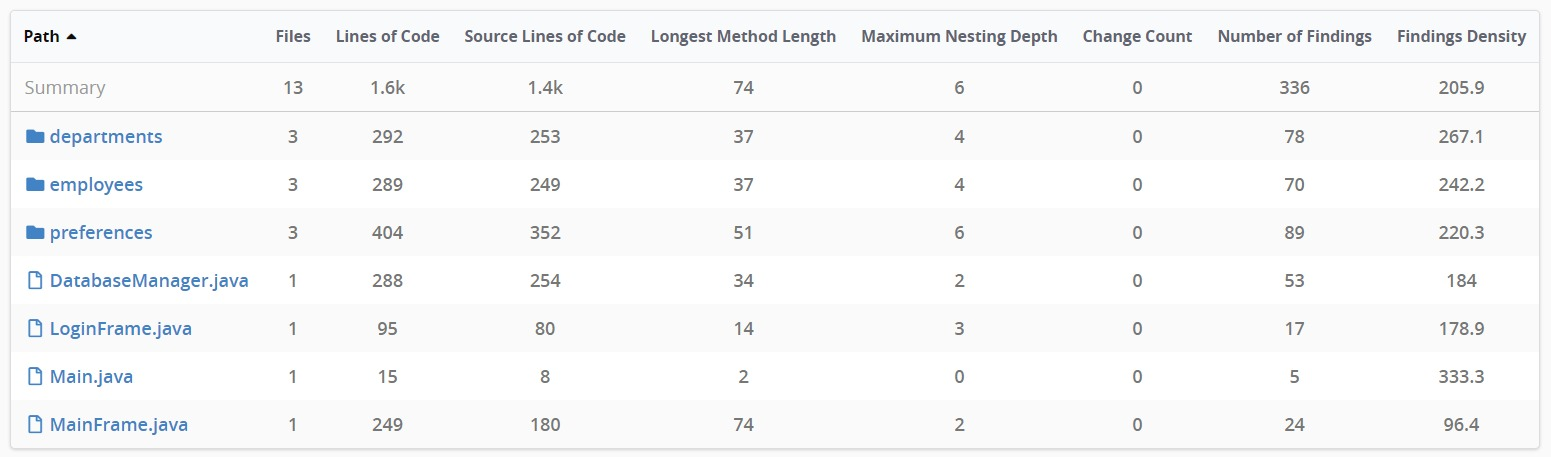
\includegraphics[width=\textwidth]{Software Metrics Before Refactoring.jpeg}
    \caption{Package Metrics of \textbf{Candidate R - Employee Payroll System} before Refactoring}
\end{figure}

\begin{figure}[h!]
    \centering
    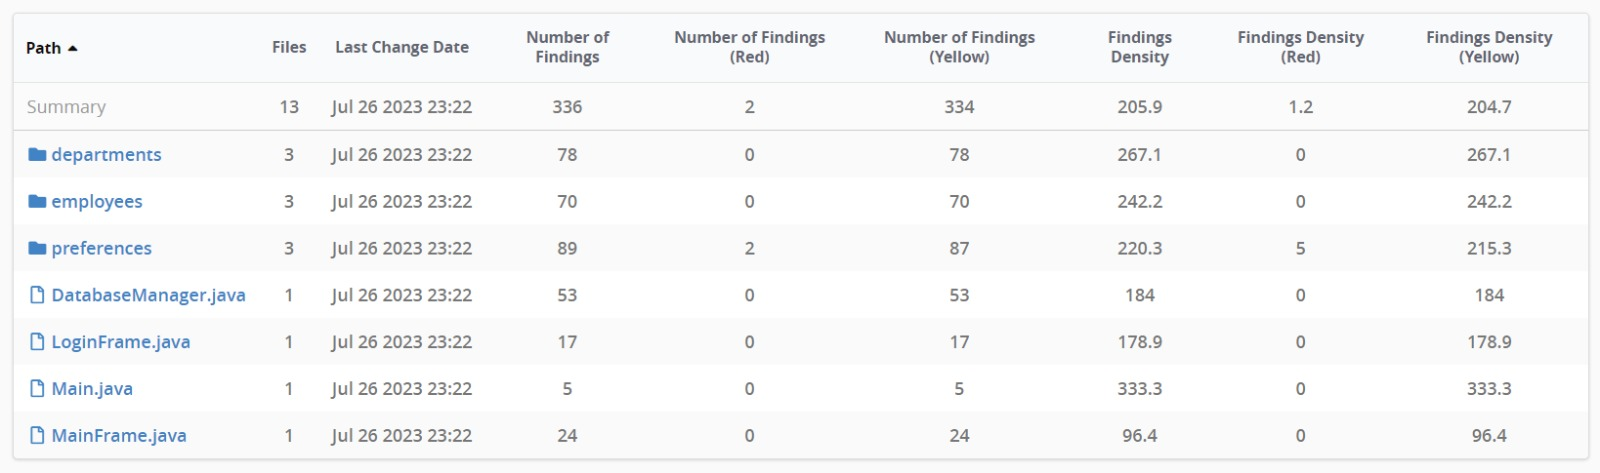
\includegraphics[width=\textwidth]{Quality Metrics Before Refactoring.jpeg}
    \caption{Quality Metrics of \textbf{Candidate R - Employee Payroll System} before Refactoring}
\end{figure}

\newpage
\subsection{After Refactoring}
\begin{figure}[h!]
    \centering
    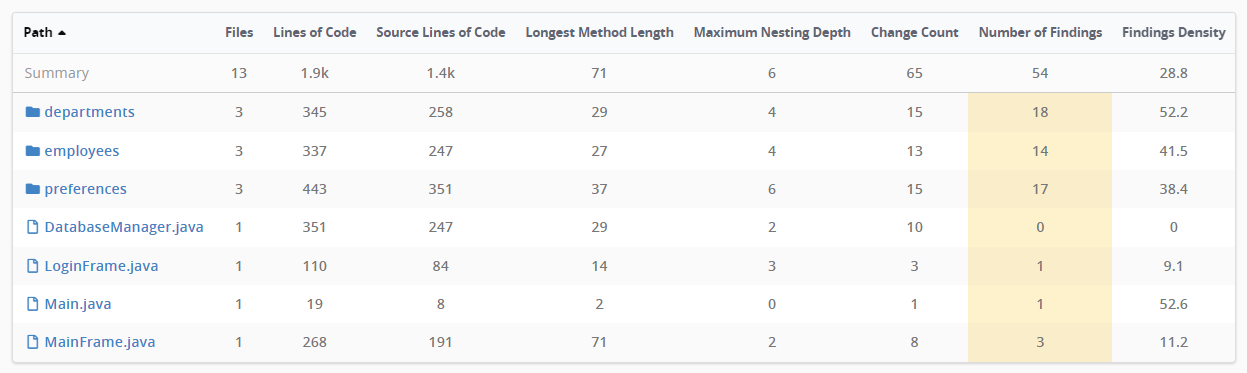
\includegraphics[width=\textwidth]{Package metrics after refactoring.png}
    \caption{Package Metrics of \textbf{Candidate R - Employee Payroll System} after Refactoring}
\end{figure}

\begin{figure}[h!]
    \centering
    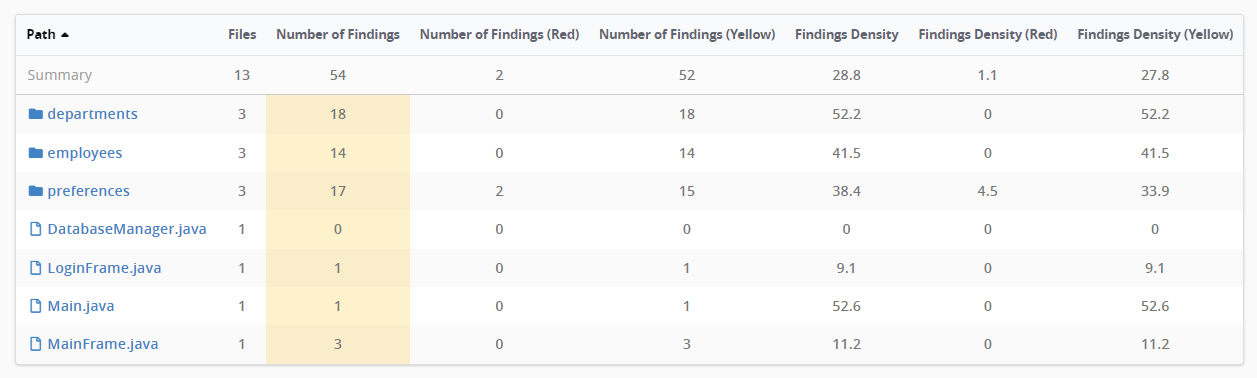
\includegraphics[width=\textwidth]{Quality metriccs after refactoring.png}
    \caption{Quality Metrics of \textbf{Candidate R - Employee Payroll System} after Refactoring}
\end{figure}

\newpage
\section{Refactoring report}

We can see the left-hand side of this final report, which has the data we initially got when we ran the system via team scale, and the right-hand side, which contains the data after refactoring. The number of lines of code has increased because we had to provide functionality for Java documentation. 

\begin{figure}[h!]
    \centering
    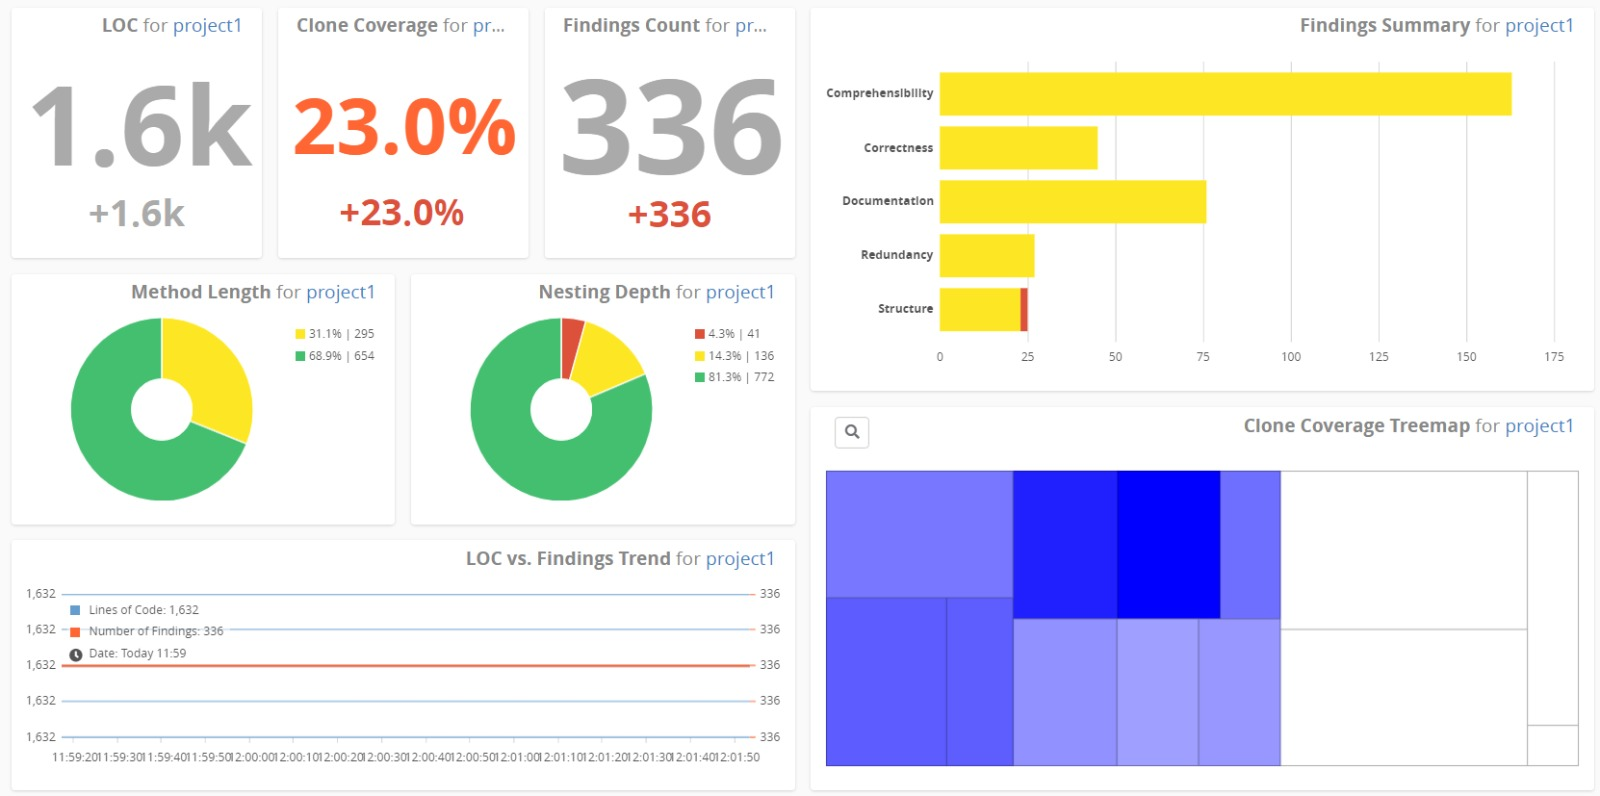
\includegraphics[width=\textwidth]{refcatoring report before.jpeg}
    \caption{Before Refactoring}
\end{figure}

\begin{figure}[h!]
    \centering
    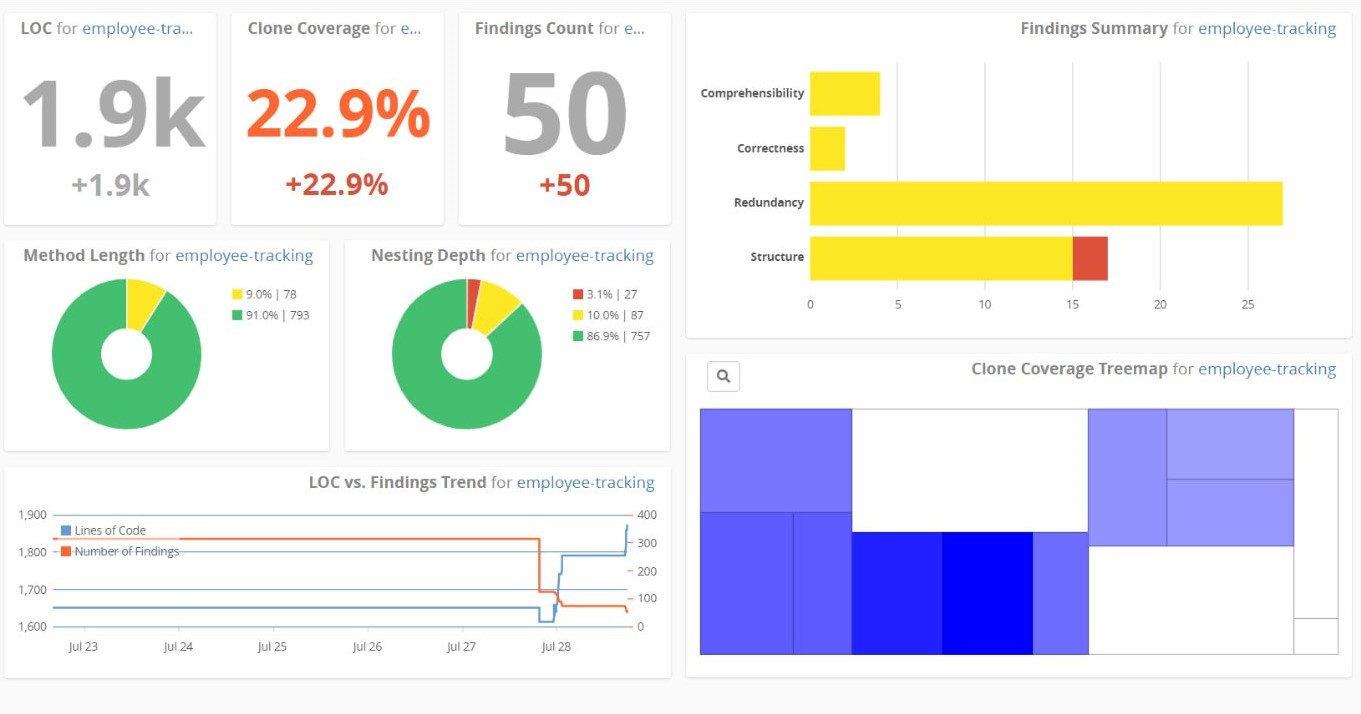
\includegraphics[width=\textwidth]{refactoring report after.jpeg}
    \caption{After Refactoring}
\end{figure}
\newpage
\begin{figure}[h!]
    \centering
    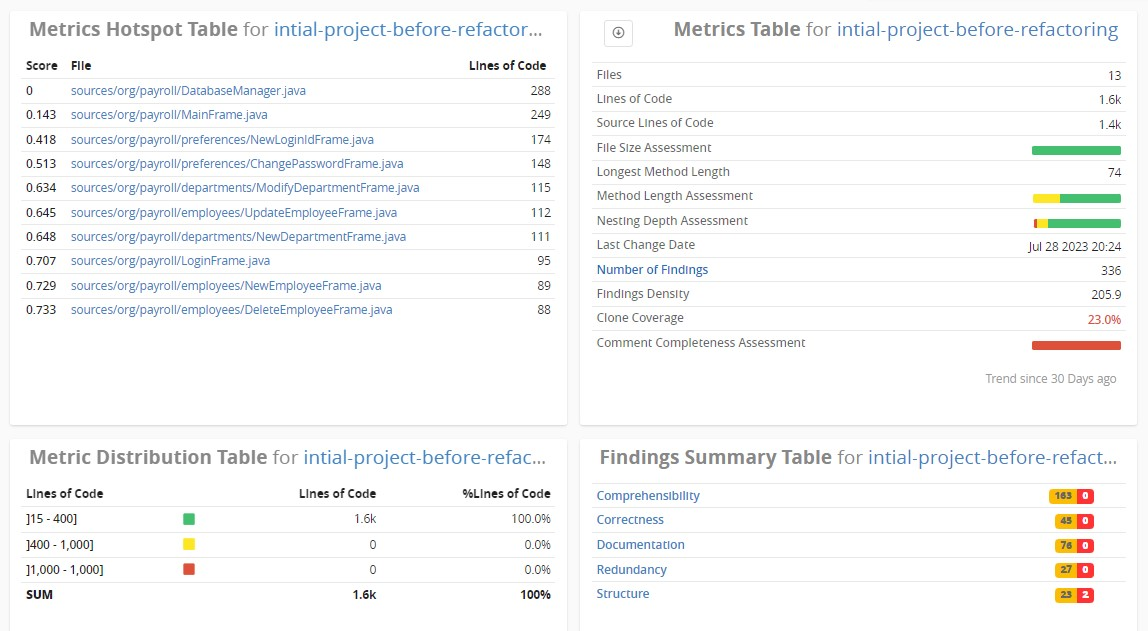
\includegraphics[width=\textwidth]{Before Refactoring Metrics.jpg}
    \caption{Software Metrics Before Refactoring}
\end{figure}
\begin{figure}[h!]
    \centering
    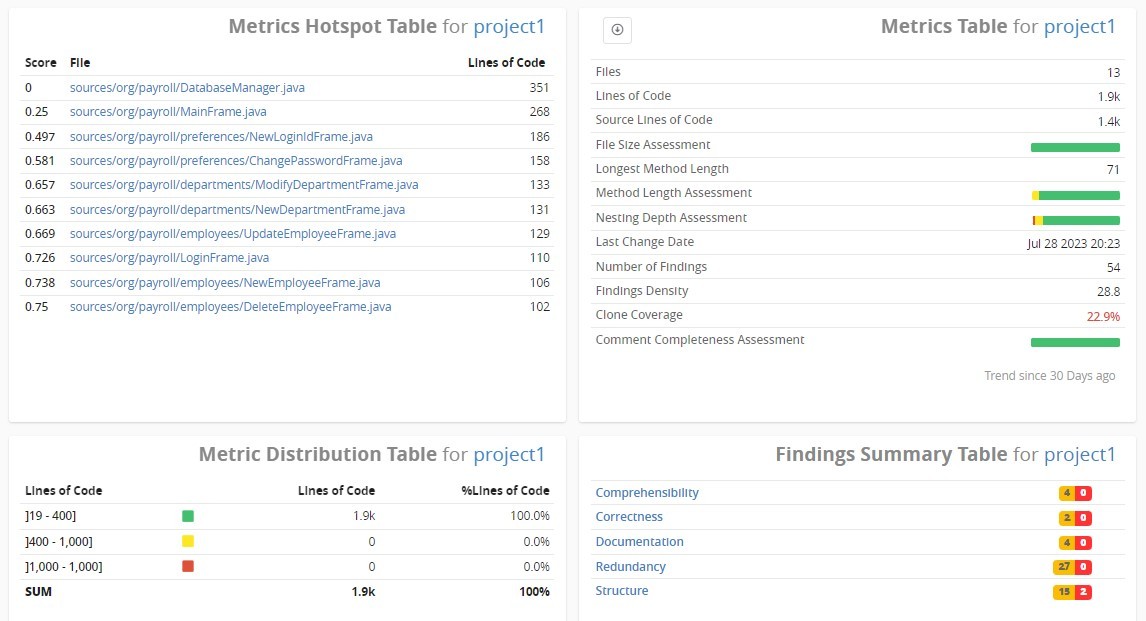
\includegraphics[width=\textwidth]{After Refactoring Metrics.jpg}
    \caption{Software Metrics After Refactoring}
\end{figure}

\newpage
\section{ Software Specifications}

 \subsection{Tools Used to Refactor the Candidate R}
    \begin{enumerate}
            \item Eclipse IDE: Eclipse is a computer programming integrated development environment. It includes a base workspace as well as other plugins that allow the system to be customised. The debuggers major feature assisted us in numerous ways in refining the code. Its fantastic user interface makes it simple for developers to debug, track, and browse through various files.

            \item TeamScale: It is a software intelligence platform that provides transparency into code quality and the underlying software development process. This allows developers, testers, and managers to better understand and manage technical debt in their systems. It is the engine for incremental analysis. Because it is directly tied to the version control system, it assesses each commit progressively. This enables TeamScale to provide timely feedback and highlight the fundamental causes of emergent problems or deteriorating trends on a commit-based basis.

            \item Sonar Lint Integration Eclipse: Sonar Lint is a free and open-source IDE extension that detects and fixes quality and security issues as you code. Sonar Lint, like a spell checker, squiggles defects and delivers real-time feedback and explicit remedial assistance to deliver clean code from the start. Nowadays, code quality is an essential component of any development pipeline. It's about preventing defects from affecting end users, preventing security risks from leaking into the wild, and making your code easier to maintain. Static Code Analysis is critical in this case.This is where Sonar Lint comes in help.

            \item Overleaf: Overleaf is a cloud-based collaborative LaTeX editor for drafting, revising, and publishing scientific publications. It collaborates with a variety of scientific publishers to provide official journal LaTeX templates as well as direct submission links.Overleaf was created by John Hammersley and John Lees-Miller, who began working on it as Write LaTeX in 2011.Write LaTeX Limited is a firm. We utilised it to document our work in Latex, and the biggest advantage is that we can share it with each team member and work simultaneously. Furthermore, the editing packages are already installed in overleaf.

            \item GIT: Git is a free and open-source distributed version control system that can handle everything from tiny to extremely large projects quickly and efficiently. Git is simple to use, has a small footprint, and delivers lightning-fast speed. It outperforms SCM tools such as Subversion, CVS, and Git. Perforce and ClearCase, for example, offer low-cost local branching, convenient staging areas, and numerous processes.



        \end{enumerate}
\newpage        
 \subsection{ Software Quality Standard to Refactor Candidate R}
 \begin{enumerate}
 
    \begin{figure}[h!]
        \centering
        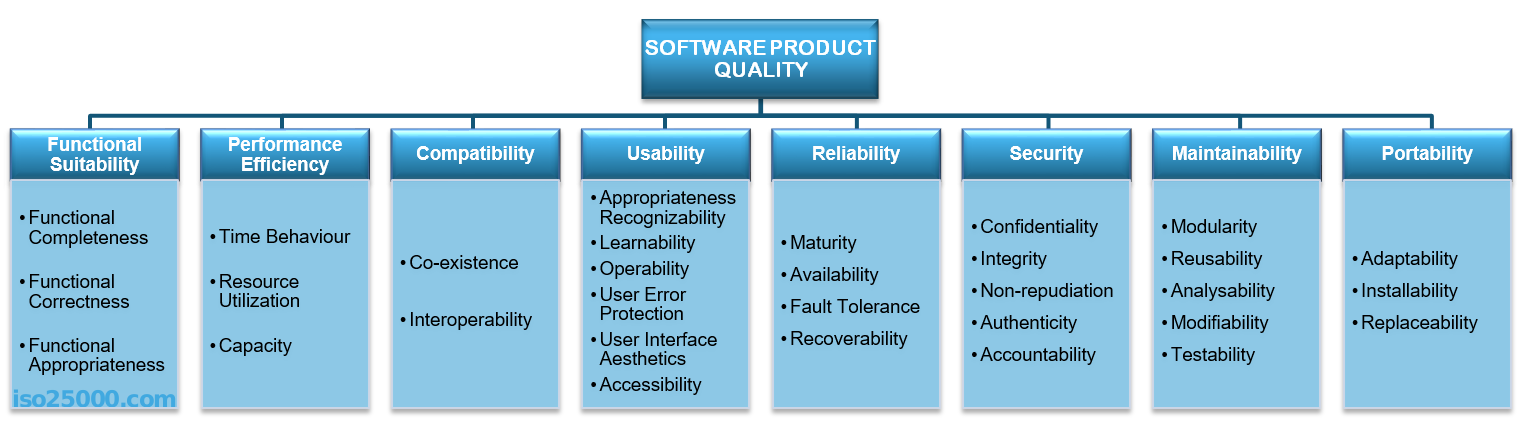
\includegraphics[width=\textwidth]{iso25010.png}
        \caption{ISO/IEC 25010:2011-Software Quality Requirements and Evaluation}
    \end{figure}
    
            \item A standard for software quality is ISO 25010, "Systems and software engineering - Systems and software Quality Requirements and Evaluation - System and software quality models."
            It outlines the models, including characteristics and sub-characteristics for both software product quality and software quality in use, and offers helpful guidance on how to use the quality models. The ISO 25010 describes two quality models:


            \item The five characteristics that make up the quality in use model, some of which are further subdivided.
            An eight-trait (each of which is further subdivided into sub-characteristics) model of product quality.


            \item Eight product quality criteria and 31 sub-characteristics make up ISO 25010: Functionality, dependability, performance effectiveness, usability, security, compatibility, maintenance requirements, and portability.

            \item According to ISO guidelines, the candidate R after refactoring must to possess the following characteristics:
            The phrase "maintenanceability" refers to how quickly a product or system may be modified to improve, correct, or adapt to changes imposed by the environment and users. We have provided a handbook that is easy for the next developer to understand, as well as a solution that is modular and easily reused.



        \end{enumerate}
\newpage
\section{Refactored source code of R}
Candidates' R source code before and after the refactoring is included in the section below, and a GitHub repository link is supplied below each of them. \\\\
Source Code of Candidate R before Refactoring \\
Link : \href{https://github.com/mahavir0/DEJA-VU---SOEN-6431-SCM/tree/master/Selected%20Source%20Code%20Repositories/Employee-Payroll-System}{https://github.com/Selected-Source-Code-Repositories/Employee-Payroll-System}\\\\
Source Code of Candidate R After Refactoring \\
Link : \href{https://github.com/mahavir0/DEJA-VU---SOEN-6431-SCM/tree/master/Candidate%20System%20Employee%20Management%20System}{https://github.com/Candidate-System-Employee-Management-System}

\section{Conclusion}
In conclusion, the software re-engineering effort aimed at improving an employee payroll system created in Java was a success. The team's comfort with the project and the code's adherence to project specifications influenced the decision to choose this system. The purpose of the re-engineering effort was to make the code more maintainable and future-proof.

\vspace{0.5cm}

The team used two code analysis tools, Teamscale and SonarLint, to detect and address flaws in the code. They chose Teamscale after comparing the results since it provided more extensive information about problems, severity levels, locations, and viable repairs, as well as better visualisations for the issues.

\vspace{0.5cm}

During the code auditing process, several undesirable errors were detected, including empty method blocks, uninitialized static variables, and naming convention violations. To address these challenges efficiently, the team used re-engineering principles and standards, with different team members taking responsibility for reworking individual problems.

\vspace{0.5cm}

The system's maintainability and functionality have improved as a result of the re-engineering initiatives. The codebase is now compliant with coding standards, and several code smells have been addressed. Furthermore, the team eliminated redundant and error-prone code practises, improving the system's overall quality.

\vspace{0.5cm}

In summary, the employee payroll system has been successfully re-engineered to improve maintainability, stability, and usability by extensive analysis, diligent reworking, and adherence to code standards. The accomplishments of the project have ensured the system's durability and increased its performance for future usage.

\newpage
\section{References}
\begin{enumerate}
    \item \href{https://users.encs.concordia.ca/~kamthan/courses/soen-6431/understanding_maintainability.pdf}{Understanding Maintainability by Dr. Pankaj Kamthan [2023]}
    \item ISO Software Quality Standard \\ \href{https://iso25000.com/index.php/en/iso-25000-standards/iso-25010}{https://iso25000.com/index.php/en/iso-25000-standards/iso-25010}
    \item TeamScale Documentation \\\href{https://docs.teamscale.com/}{https://docs.teamscale.com/}
    \item Improving Code Quality Using Teamscale \\\href{https://docs.teamscale.com/introduction/improving-software-quality/}{https://docs.teamscale.com/introduction/improving-software-quality/}
    \item Teamscale Integration for Eclipse \\\href{https://docs.teamscale.com/getting-started/eclipse/}{https://docs.teamscale.com/getting-started/eclipse/}
    \item Integrating Sonar to Eclipse \\\href{https://subscription.packtpub.com/book/programming/9781849517867/6/ch06lvl1sec03/integrating-sonar-to-eclipse#:~:text=Launch%20Eclipse%20and%20go%20to,hosted%20at%20the%20preceding%20address.}{https://subscription.packtpub.com/book/programming/integrating-sonar-to-eclipse}
    \item Catching Issues in the IDE with SonarLint \\\href{https://docs.sonarcloud.io/improving/sonarlint/#:~:text=SonarLint%20is%20a%20free%20IDE,the%20code%20is%20even%20committed.}{https://docs.sonarcloud.io/improving/sonarlint/}
    \item Everything you need to know about Code Smells \\ \href{https://www.codegrip.tech/productivity/everything-you-need-to-know-about-code-smells/}{https://www.codegrip.tech/productivity/everything-you-need-to-know-about-code-smells/}
    \item ISO/IEC 25010 Software Quality Model
    \\\href{https://blog.codacy.com/iso-25010-software-quality-model//}{https://blog.codacy.com/iso-25010-software-quality-model/}
    \item Manage Team's Project on Trello \\ \href{https://trello.com/invite/b/7KgMwndv/ATTI48a736897511bb8c57c1553f7b0e772dCBC3EF6B/soen-6431}{https://trello.com/soen-6431}
\end{enumerate}
    
\end{document}